% Preamble
% --------
\documentclass[12pt]{article}

\newcommand{\codename}[0]{\texttt{apex-sim}~}

% Packages
% --------
\usepackage{blindtext} %for boilerplate text (\blindtext)
\usepackage{geometry} %for paper dimensions and margins
\usepackage{graphicx} % for including graphics
\usepackage{hyperref} % for hyperlink support
\usepackage{todonotes}

% Page Setup
% ----------
\geometry{letterpaper, margin=1in}

% Title content and formatting
% ----------------------------
\title{Apex Instruction Set Architecture Simulator (\texttt{apex-sim}) \\ Phase 2 Documentation}
\author{Matthew Cole \\ \texttt{mcole8@binghamton.edu}
\and
Brian Gracin \\ \texttt{bgracin1@binghamton.edu}}
\date{19 November 2016}

\begin{document}
% Emit title content
% ------------------
\pagenumbering{gobble}
\maketitle
\tableofcontents
\newpage
\listoffigures
\listoftables
\newpage
\pagenumbering{arabic}

%---------------

\section{Design}
\codename is a simulator for the \textit{Architecture Pipeline EXample} (APEX) Instruction Set Architecture (ISA).
\codename consists of the following components:
\begin{itemize}
  \item \texttt{main.cpp} contains the driver program. The driver program provides file input for instructions, user interface operations, maintaining persistent simulator state and statistics monitoring. This component is discussed in section \ref{sec:driver}.
  \item \texttt{apex.cpp} contains helper functions for \texttt{main.cpp}. These include wrapper functions that delegate interface actions down to individual classes.
  \item Several source files provide the objects modeling components of the pipeline. These components are discussed in section \ref{sec:classes}. Briefly, they are
	\begin{itemize}
		\item \texttt{code.cpp} models the simulator's read-only instructions file.
		\item \texttt{cpu.cpp} (plus its associated helper functions in \texttt{simulate.cpp}) models the stages in the pipeline and interact with the Instruction Queue (IQ) and Reorder Buffer (ROB). It is responsible for overall execution of a single cycle through its helper function \texttt{simulate}. 
		\item \texttt{data.cpp} models the simulator's read-write main memory.
		\item \texttt{iq.cpp} models the simulator's IQ.
		\item \texttt{registers.cpp} models the simulator's unified register file.
		\item \texttt{stage.cpp} models a single stage in the pipeline. It also doubles as an inflight instruction or entry in the IQ or ROB. This allows advancement of an inflight instruction to be greatly simplified.
	\end{itemize}
	\item \texttt{simulate.cpp} provides the functions that allow the CPU to simulate working on each of its stages, inter-stage communication through advancement, stalls for basic inter-stage interlocks, out-of-order execution and reordering, and forwarding. These implementation details are described in section \ref{sec:implementation}.
\end{itemize}
Figure \ref{fig:overview} shows class interactions and data flow between each of the stages and support classes.
Finally, we discuss our team's work log in section \ref{sec:worklog}.

\begin{figure}
  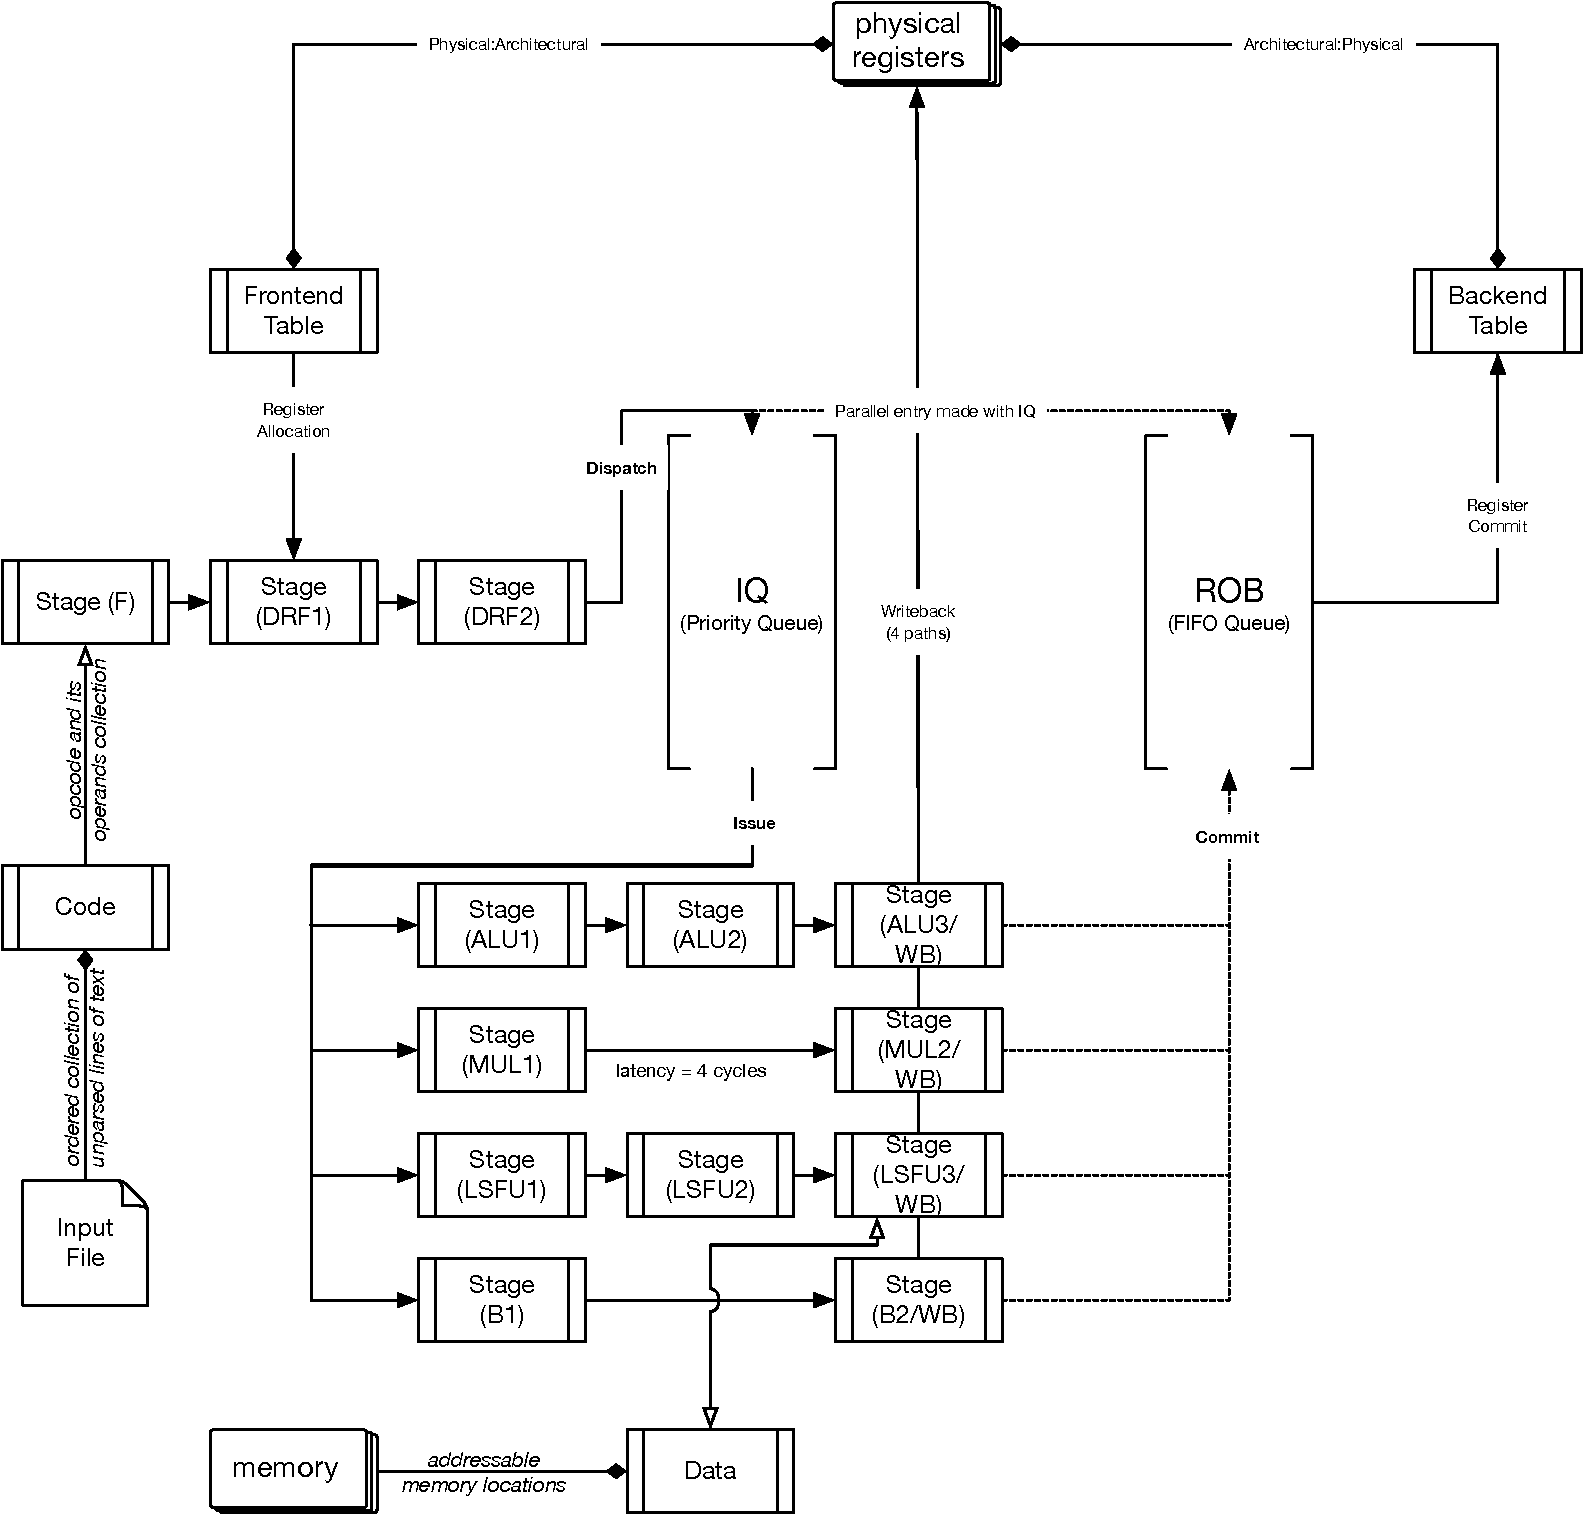
\includegraphics[width=\linewidth]{./figs/apex-sim-overview-2.pdf}
  \caption{APEX pipeline and class data flows.}
  \label{fig:overview}
\end{figure}

\subsection{Driver Program}
\label{sec:driver}
The \codename entry point file is \texttt{main.cpp}. Besides maintaining simulator state variables for the current cycle, program counter and instructions filename, this program shepherds execution through the lifecycle of the program and provides a user interface for interacting with the simulator. The functionality of the driver program is as follows:
\begin{enumerate}
  \item Verify sanity of command line inputs (lines 23-32).
  \item Instantiate class instances for the simulator (lines 34-40).
  \item Perform the initialization of each pipeline stage (line 43).
  \item Prepare and begin the simulator user interface's operations (lines 48-54).
  \item Parse user interface inputs and delegate actions to interface helper functions (lines 57-127).
\end{enumerate}

\texttt{main.cpp} also provides helper functions which delegate work down to class instances in \texttt{apex.cpp}. These functions are:
\begin{itemize}
  \item \texttt{help()} displays the user interface keyboard shortcuts. It's invoked at startup, on request from the user, and whenever the user provides an input which is not recognized.
  \item \texttt{initialize()} resets the simulator state, and invokes the class instances' own \texttt{\textit{classname}.initialize()} functions which reset the instances' internal state.
  \item \texttt{display()} displays the simulator internal state variables as well as delegated calls to each class' \texttt{\textit{classname}.display()} function.
  \item \texttt{stats()} displays simulator execution statistics.
  \item \texttt{simulate()} is the most important of the helper functions. It is responsible for controlling simulation of the \texttt{CPU.simulate()} function for a given number of cycles, and allowing the CPU class to communicate that it has encountered an error, reached EOF of a code file without a HALT instruction, or has processed a HALT instruction through the pipeline.
  \item \texttt{quit()} gracefully halts the simulator and triggers a final call to \texttt{display()}.
\end{itemize}

\subsection{Classes}
\label{sec:classes}
\codename models each major component of the APEX system as a standalone class. Unless mentioned below, these classes did not change appreciably from release v1.0 and are not discussed further in this report. Please see the release v1.0 documentation for discussion of these unchanged classes.

\subsubsection{Issue Queue}

\subsubsection{Reorder Buffer}

\subsubsection{Data}

\subsubsection{Registers}

\subsubsection{CPU and Stages}


%-----------------------
\section{Implementation}
\label{sec:implementation}
In this section, we will discuss key aspects of our simulator's execution: the stage-wise reverse-ordered execution, register renaming, dispatch, issue, commit, register value forwarding.

\subsection{Reverse-Ordered Execution}

\subsubsection{Committing}


\subsubsection{Advancing}

\subsubsection{Working}

\subsubsection{Forwarding}
\todo{Add table of forwarding scenarios.}
\begin{table}
  \centering
  \caption{APEX Forwarding Scenarios}
  \label{tab:fwdscenarios}
  \begin{tabular}{l|l|c}
    Source Stage & Destination Stage & Description\\
    \hline
    - & - & - \\
  \end{tabular}
\end{table}

\todo{Add discussion of forwarding from writeback stages.}

\begin{table}
  \centering
  \caption{APEX Instruction Source and Destination Sets}
  \label{tab:instsets}
  \begin{tabular}{l|c|c}
    Instruction & Destination Set Operand Indices & Source Set Operand Indices\\
    \hline
    Arithmetic					 	& 0 & 1,2\\
    MOVC 							& 0 & - \\
    LOAD							& 0 & 1 \\
    STORE							& 1 & 0 \\
    BAL, JUMP						& - & 0 \\
    BZ, BNZ 						& - & - \\
    HALT, NOP						& - & - \\
  \end{tabular}
\end{table}

\subsection{Register Renaming and Allocation}
\subsubsection{Allocation}
\todo{Add discussion of allocating in ascending order of tag. See para 5 in spec.}
\subsubsection{Renaming}

\subsection{Dispatch}
\subsubsection{Stalling for Multiple Control Flow Instructions}

\subsection{Issue}
\todo{Add discussion of issuing LSFU in program order. See para 4 in spec.}

\subsection{Commit}
\todo{Add discussion of how commit logic works.}

\subsection{Statistics}
\todo{Add discussion of statistics mechanism in apex.cpp, used in simulate.cpp}


%-------------------
\section{Work Log}
\label{sec:worklog}
We open-sourced \codename under the MIT license, and developed it using a GitHub repository. \footnote{The repository is available at \url{https://github.com/colematt/apex-sim}}
This repository contains this documentation, all source code, reference materials on the APEX ISA semantics, and other related materials.
Additionally, it contains an in-depth look at our work progress over the course of this project at a much finer grain than this report contains.
As of writing this report, \todo{Add number of commits} commits were made with a total of \todo{Add number of lines of code} lines of code.
Naturally, such a volume of code and the required levels of collaboration would have been nearly impossible without the use of some sort of repository.
We encourage the curious reader to see these statistics in depth using the \textbf{Pulse} and \textbf{Graphs} tabs available on the repository.

Table \ref{tab:worklog} is a broad, chronological overview of work performed by each member.

\begin{table}
\centering
\caption{Chronological Work Log}
\label{tab:worklog}
\begin{tabular}{l|p{2.75in}|p{2.75in}}
Date         	& Matthew's Task
				& Brian's Task \\
\hline
Dec 5, 2016  	& Moved source files into their own directory, updated Makefile.
				& Began modifying Registers class to support URF operations. Created Front-end, Back-end table, Free-list. Prototyped API functions to class. \\
Dec 6, 2016  	& Updated UI for new commands specified in Phase 2. Added stats mechanisms. Updated display methods.
				& Further work on Registers class, updated function to create new instances of registers. Began work on ROB class. \\
Dec 7, 2016		& Allowed templating Stages to IQ and ROB deques. Continued work on final report.
				& Completed ROB and IQ class architectures. Added commit and head-compare utility functions to ROB and IQ for programmer convenience. \\
Dec 8, 2016		& Visibility and inter-class communications pathways. Added halting logic.
				& Initial compilation and end-to-end testing. Added issue utility function to IQ for programmer convenience. \\
Dec 9, 2016		& Continued work on documentation.
				& Continued work on documentation.\\
Dec 10, 2016	& Continued work on documentation. Fixed blocking for advance functions. Began work phase code for all FUs.
				& Completed issue, committing and writeback design. Extensive end-to-end troubleshooting.\\
Dec 11, 2016	& Finalized Work phase, Advancing phase and Forwarding phase in \texttt{simulate()} function. Squashed 3 issues.
				& Continued troubleshooting on all classes.\\
Dec 12, 2016	& Completed final report, troubleshooting, screen captures and submission package.
				& Substantial troubleshooting and \textbf{Checkpointed Release v.2.0!}\\
\end{tabular}
\end{table}

%---------------
\newpage
\appendix
\section{Appendix: Screen Captures}
\todo{Add screen captures.}
\end{document}
